\documentclass[12pt]{article}
\usepackage{amsmath, amssymb}
\usepackage{graphicx}
\usepackage{float}
\usepackage[letterpaper, margin=1in]{geometry}
\usepackage[colorlinks=true, linkcolor=blue, urlcolor=blue]{hyperref}
\usepackage{listings}
\usepackage{booktabs}
\usepackage{siunitx}
\usepackage{booktabs, xcolor, colortbl, array, caption}
\usepackage{lettrine}
\usepackage{bm}

\definecolor{headerblue}{RGB}{50, 90, 130}
\definecolor{rowshade}{RGB}{245, 248, 252}
\definecolor{accentgold}{RGB}{180, 140, 50}



\begin{document}
\pagestyle{empty}
\begin{center}
    \Huge \textbf{Plan}
\end{center}

I obtained my data from \href{https://www.baseball-reference.com}{Baseball Reference}. I went to Shohei's game logs and copied the batting game logs for each year from 2021 to 2023. I created the unintentional walks column by subtracting intentional walks from intentional walks, and the singles column with 1B = H - (2B + 3B + HR). I used the formula to calculate wOBA from this. These game logs contain a position column, which I used to distinguish between games he pitched in and didn't. Since multiple positions can be played in a game (for example, in a start, he'd exit the game after a certain number of innings, and would play DH for the rest of the games), I split the position on each space and found which lists contained ``P''. I then split the dataset into two datasets, one in which Shohei pitched and one in which he didn't.

\begin{table}[ht]
    \centering
    \setlength{\tabcolsep}{12pt}
    \renewcommand{\arraystretch}{1.35}
    \begin{tabular}{%
            >{\bfseries\small}l
            >{\small\centering\arraybackslash}c
            >{\small\centering\arraybackslash}c
            >{\small\centering\arraybackslash}c}

        \toprule
        % \rowcolor{headerblue!12}
        \textbf{Statistic}
                   & {\textbf{Pitching}}
                   & {\textbf{Not Pitching}}
                   & \textbf{Overall}                        \\
        \midrule

        Count      & 68                      & 363   & 431   \\
        \rowcolor{rowshade}
        Mean       & 0.381                   & 0.398 & 0.395 \\
        Std.\ Dev. & 0.335                   & 0.290 & 0.297 \\
        \rowcolor{rowshade}
        Min        & 0.000                   & 0.000 & 0.000 \\
        25\%       & 0.175                   & 0.174 & 0.174 \\
        \rowcolor{rowshade}
        Median
                   & 0.294                   & 0.352 & 0.345 \\
        75\%       & 0.565                   & 0.568 & 0.566 \\
        \rowcolor{rowshade}
        Max        & 1.422                   & 1.372 & 1.422 \\

        \bottomrule
    \end{tabular}
    \caption*{\textbf{wOBA summary statistics}}
\end{table}

\begin{figure}[H]
    \centering
    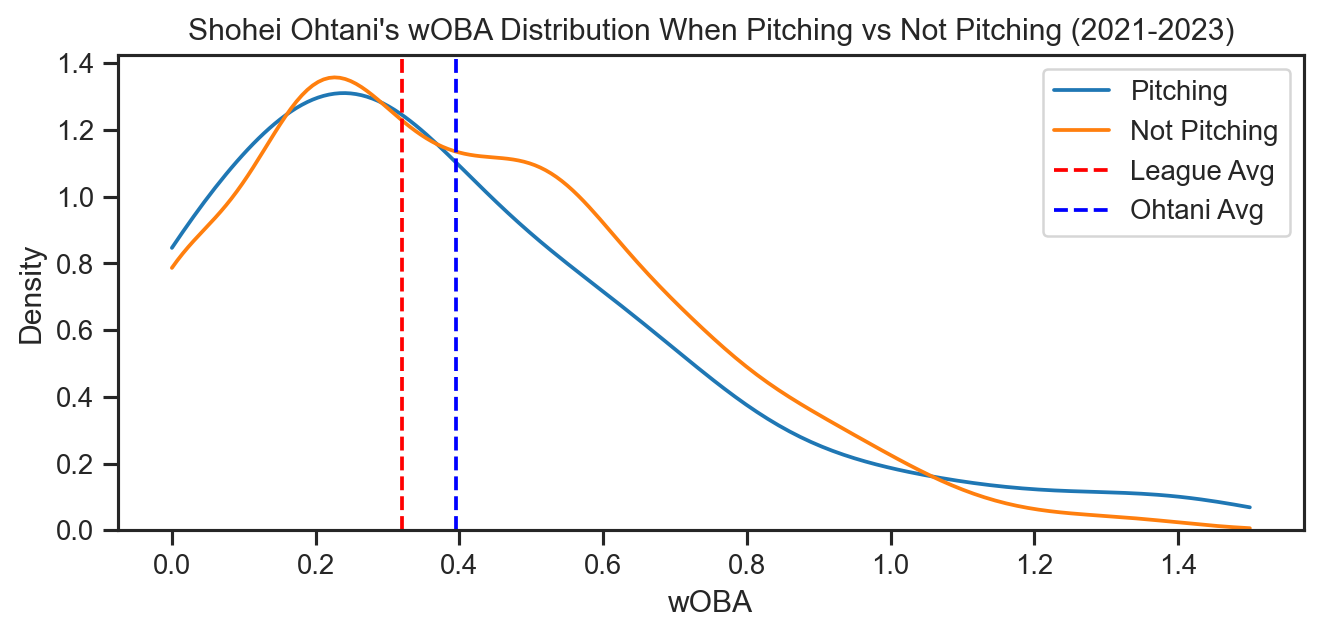
\includegraphics[width=1\textwidth]{woba_dist.png}
\end{figure}

\begin{figure}[H]
    \centering
    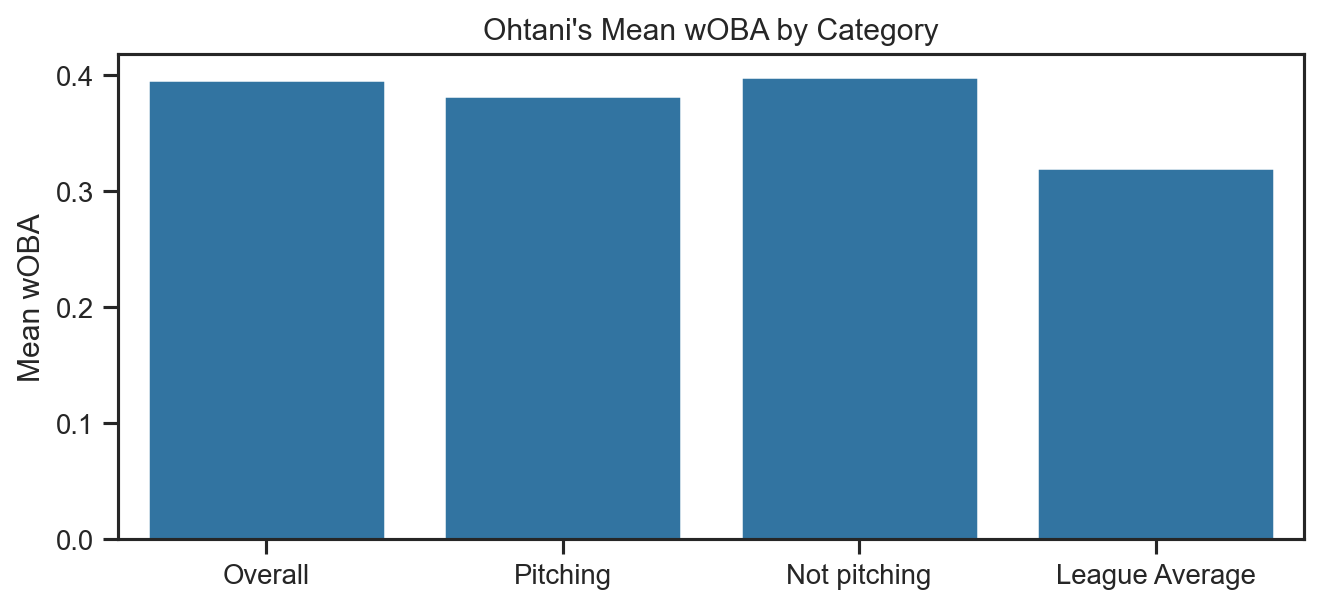
\includegraphics[width=1\textwidth]{woba_bar_chart.png}
\end{figure}



The mean wOBA is 0.398 when not pitching compared to 0.381 when pitching, and the median is 0.352 versus 0.294, showing slightly higher values when not pitching. His mean wOBA regardless of position is 0.395, which is 0.075 higher than the league average wOBA (a substantial increase, as the standard deviation is roughly .040). This indicates that Shohei does in fact perform better when not pitching. It also shows that both distributions are right skewed, as the mean is greater than the median for each, which supports the density plot. The standard deviation for pitching is higher than when not pitching (\(s_p = 0.335 > s_{np} = 0.280\)), as is the range (\(1.422 > 1.372\)), indicating higher variability. This can likely be explained by the smaller sample size (\(n_p = 68 < n_{np} = 363\)). \textbf{So, it appears that while Shohei performed slightly better when pitching compared to when not pitching, it is likely not statistically significant}, due to the smaller sample size when pitching and the fact that the standard deviations for each is much bigger than the difference in means.  \textbf{\(\bm{H_0}\) is unlikely to be rejected.}

We'll test this, but first, the conditions for inference must be met. First, the pitching data is a random sample from the previously discussed larger, theoretical population of all games Shohei could have pitched in; the not pitching data is also a random sample from the population of all games that Shohei could have batted but not pitched in. Second, since this population is theoretically unlimited, the 10\% conditions are met for both (\(\frac{1}{10}\infty = \infty > n_p = 68 \text{ and } n_{np} = 363\)). Last, the CLT applies to both, as \(n_p = 68 \geq 30\) and \(n_{np} = 363 \geq 30\), meaning both sampling distributions are approximately normal. Therefore, the conditions for inference are met.
\end{document}